\section{Bahnplanung}
\subsection{Bewegungsarten}
\begin{minipage}{0.5\linewidth}
    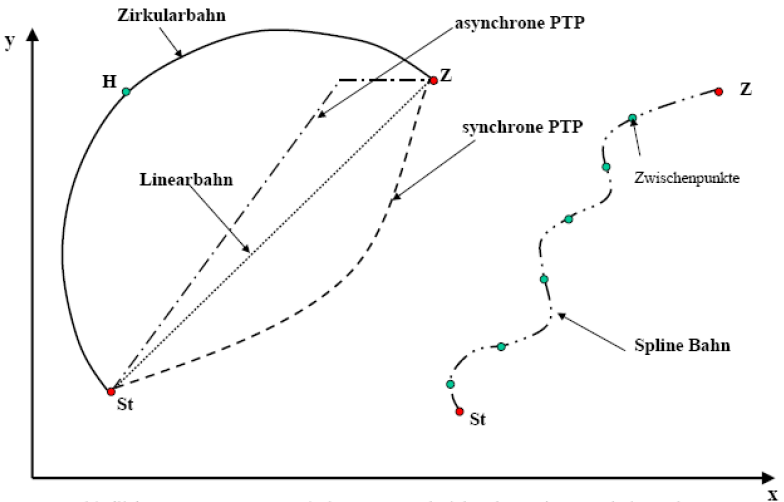
\includegraphics[width=\linewidth]{./bilder/bewegungsarten.png}
\end{minipage}
\begin{minipage}{0.5\linewidth}
    \includegraphics[width=\linewidth]{./bilder/Bewegunggreifer.png}
\end{minipage}

\begin{minipage}{0.5\linewidth}
    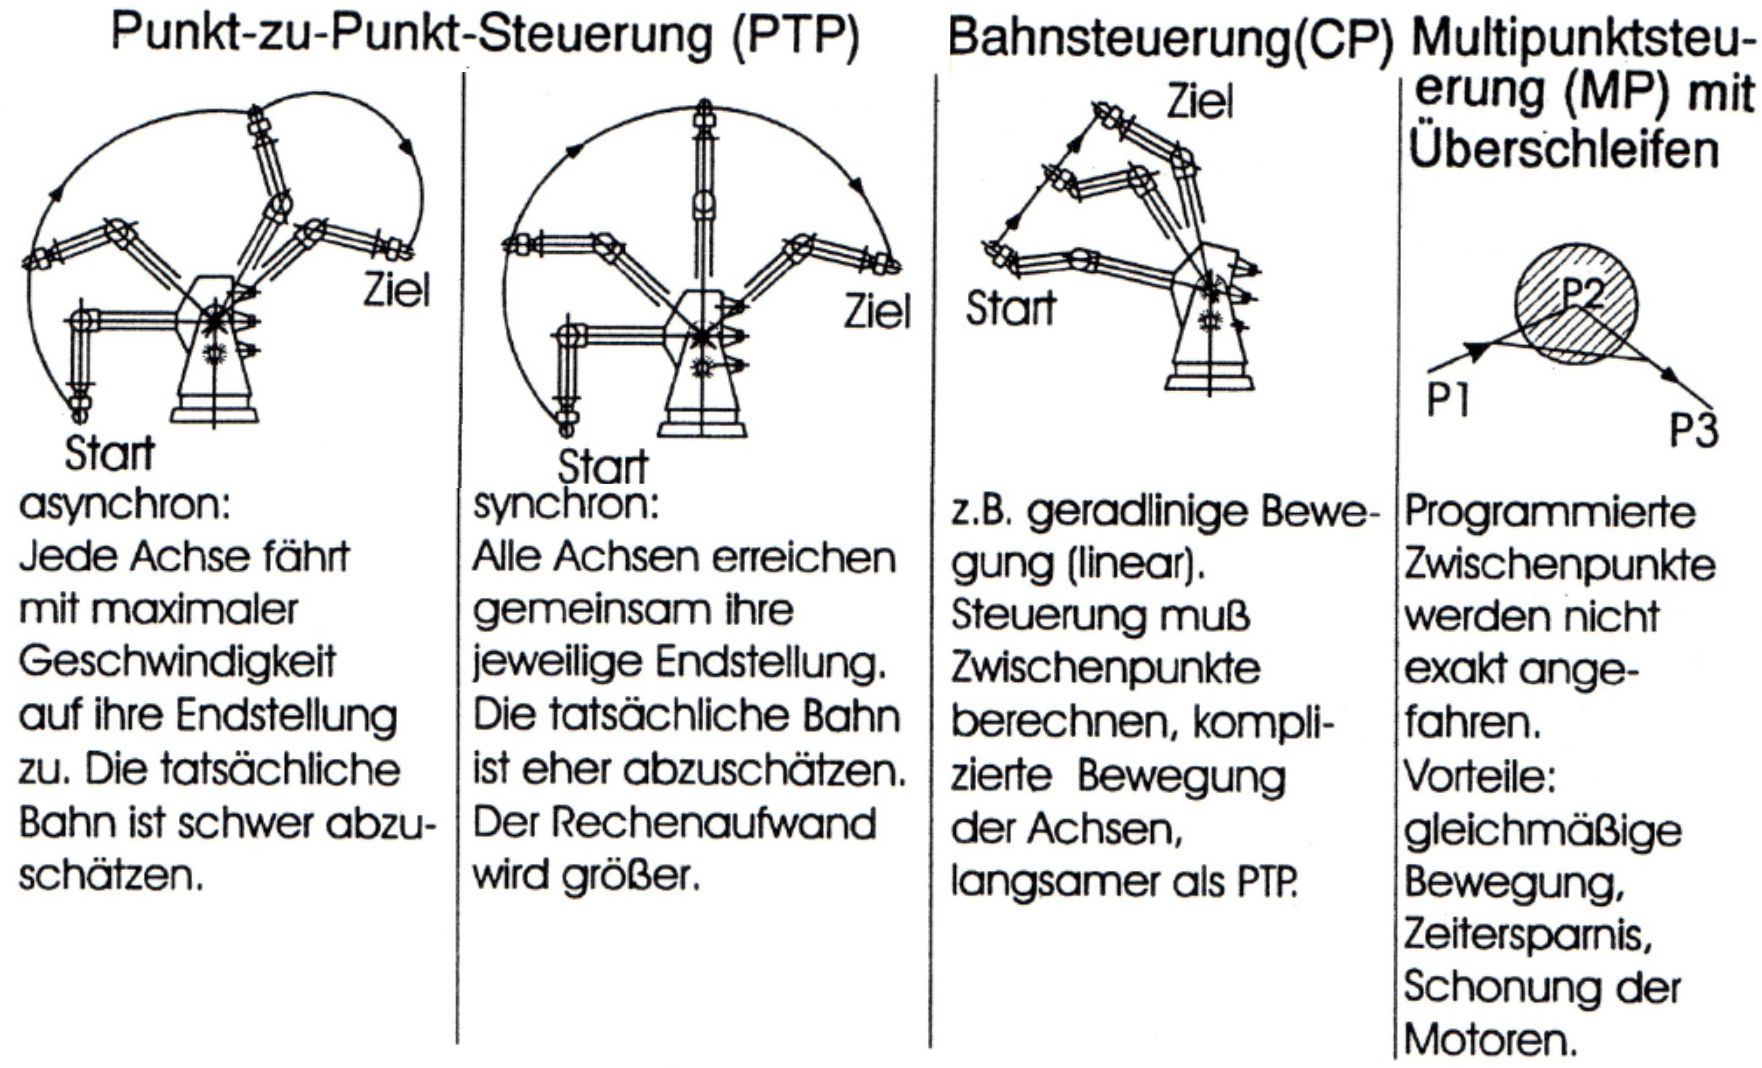
\includegraphics[width=\linewidth]{./bilder/bewegungsarten2.png}
\end{minipage}
\begin{minipage}{0.5\linewidth}
    \begin{itemize}
        \item  \textbf{asynchronen PTP}
        \begin{itemize}
            \item  Jede Achse verfährt vollständig unabhängig von anderen Achsen.
        \end{itemize}
        \item  \textbf{synchronen PTP}
        \begin{itemize}
            \item  Wird durch die Achse mit der grössten Bahndauer bestimmt.
            \item Die Geschwindigkeit der anderen Achsen wird reduziert,so dass alle gleichzeitig ihren Endpunkt erreichen.
        \end{itemize}
        \item  \textbf{vollsynchronen PTP}
        \begin{itemize}
            \item  Nicht nur die Bahnzeiten für die Gelenke synchronisiert.
            \item Auch Beschleunigungs und Brmezeiten synchron.
        \end{itemize}
    \end{itemize}
\end{minipage}
\vspace{-1cm}
\subsubsection{Singularität}
\begin{minipage}{0.5\linewidth}
    \textbf{Singuläre Konfiguration}
    \begin{itemize}
        \item Mehrere Achsen liegen in einer Linie
        \item Die Drehung einer Achse kann durch Gegendrehung einer anderen Achse kompensiert werden.
        \item Ein Freiheitsgrad geht verloren, da für eine Drehachse zwei Gelenke verwendet werden.
    \end{itemize}
\end{minipage}
\begin{minipage}{0.5\linewidth}
    \textbf{Grenzsingularität}\newline
    \begin{itemize}
        \item Der Roboter ist ganz ausgestreckt oder an einer Position am Rande seines Arbeitsraum
        \begin{itemize}
            \item Es gibt Richtungen in die er sich nicht mehr bewegen kann
        \end{itemize}
    \end{itemize}
\end{minipage}

\subsection{Bahnüberschleifen}
Vorteile:
\begin{itemize}
    \item[+] Zeitgewinn
    \item[+] Vermeidung von ruckartigen Bewegungen
    \item[+] Hindernisumfahrung durch Definition von Zwischenpunkten 
\end{itemize}

\begin{minipage}{0.345\linewidth}
    \textbf{PTP}\newline
    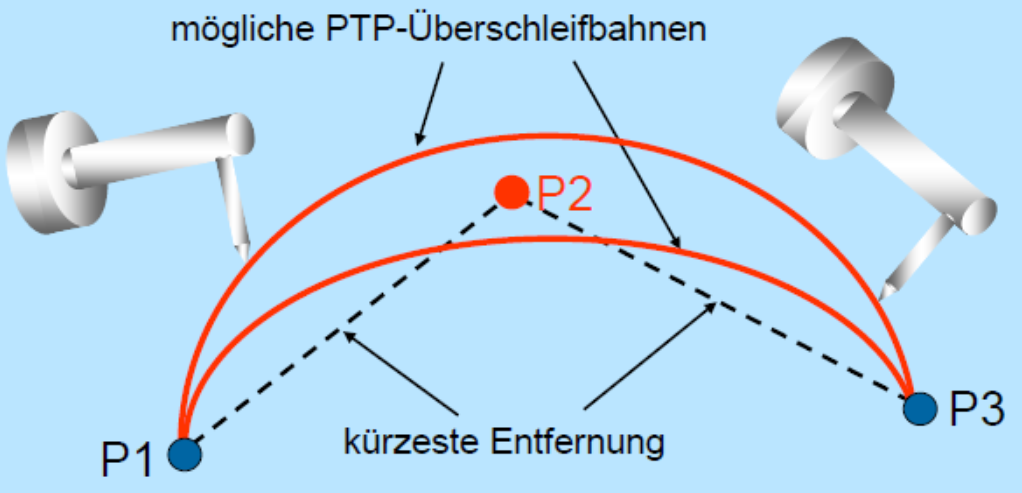
\includegraphics[width=\linewidth]{./bilder/UeberschleifenPTP.png}
\end{minipage}
\begin{minipage}{0.32\linewidth}
    \textbf{Linear}\newline
    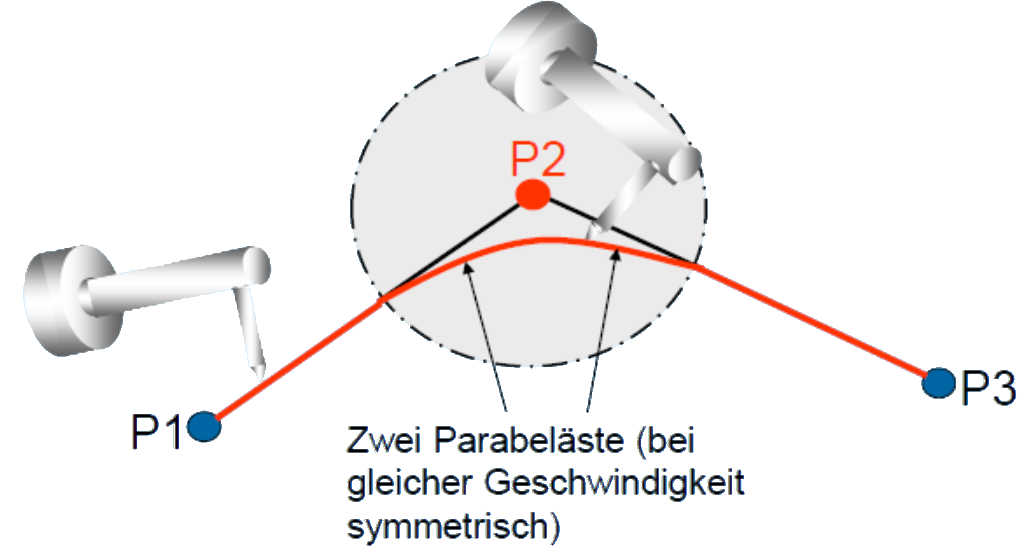
\includegraphics[width=\linewidth]{./bilder/UeberschleifenLin.png}
\end{minipage}
\begin{minipage}{0.32\linewidth}
    \textbf{Zirkular}\newline
    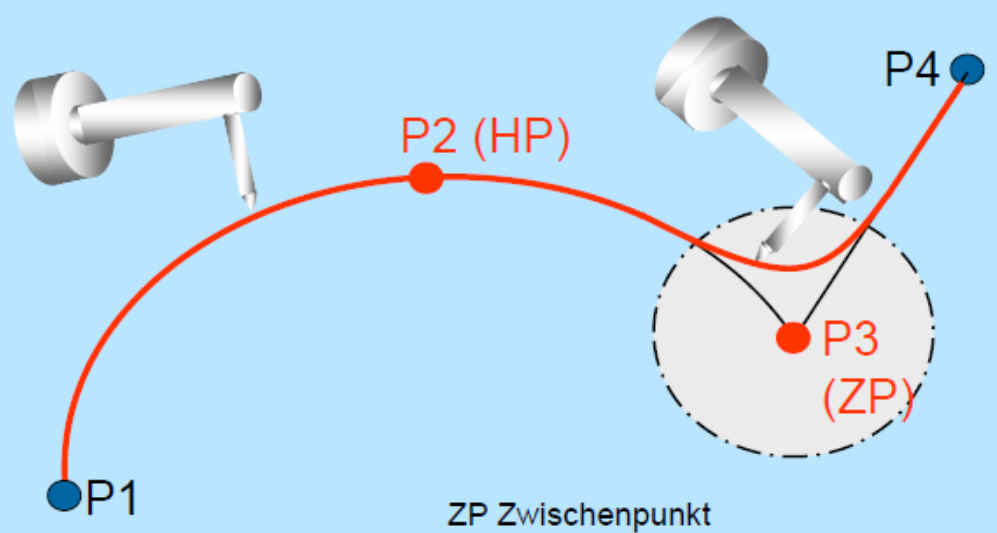
\includegraphics[width=\linewidth]{./bilder/UeberschleifenCirc.png}
\end{minipage}

\subsection{Bahnerzeugungn in Gelenkkoordinaten}
\begin{multicols}{2}
    \begin{itemize}
        \item[+] Minimale Bewegung bei jedem Gelenk.
        \item[+] Max. Geschwindigkeit und max. Momente bekannt.
    \end{itemize}

    \begin{itemize}
        \item[-] Bahngeometrie in kart. Raum unbekannt.
        \item[-] Kollisionsvermeidung schwierig.
    \end{itemize}
\end{multicols}

\subsubsection{Kubisches Polynome}
\begin{tabular}{ll}
\multicolumn{2}{l}{\textbf{Bedingungen}}\\
$ \theta(0)=\theta_0 $& $ \theta(t_f) = \theta_f$\\ 
$ \dot{\theta}(0)=0 $& $ \dot{\theta}(t_f) = 0$\\
\multicolumn{2}{l}{\textbf{Gleichung}}\\
\multicolumn{2}{l}{$ \theta(t)=a_0 + a_1t + a_2t^2+a_3t^3$}\\
\multicolumn{2}{l}{\textbf{Koeffizienten}}\\
$a_0= \theta_0$&$a_1=0 $\\
$a_2 = \frac{3}{t_f^2}(\theta_f - \theta_0) $&$a_3=-\frac{2}{t_f^3}(\theta_f-\theta_0) $\\
\end{tabular}
\paragraph{Bsp.}
Ein Roboter mit einer Rotationsachse ($\theta$) soll sich von $\theta$= -5\textdegree bis zu $\theta$= 80\textdegree in 4 Sekunden bewegen.\newline
Gesucht: Koeff des kubischen Polynoms, max Geschwindigkeit und max Beschleunigung der Achsen.
Stellen sie die Position Grafisch dar.

\begin{tabular}{ll}
    Kubisches Polynom & $\theta(t)=a_0 + a_1t + a_2t^2+a_3t^3$\\
                        & $a_0 = -5$\textdegree$,\; a_1=0,\; a_2=15.93,\; a_3=-2.656 $\\
    Geschwindigkeit     & $\dot{\theta}=a_1+2a_2\cdot t+3a_3 \cdot t^2 $\\
                        & $ \qquad 31.86 \cdot t - 7.968 \cdot t^2$\\
    Beschleunigung      & $ \ddot{\theta}=2a_2 + 6a_3 \cdot t$\\
                        & $ \qquad 31.86 - 15.936 \cdot t$\\
    $\rightarrow \ddot{\theta}=0 $ & t = $\frac{31.86}{15.936}=2s$\\
    max. Geschw.        & $ \dot{\theta}_{max}= 31.86\cdot 2s - 7.968\cdot 4s = 31.848$\textdegree$ /s$\\
    max. Besch.         &$ \ddot{\theta}_{max} \rightarrow t=0 $ \\  
                        &$ \ddot{\theta}_{max} \rightarrow t=t_f $ \\              
\end{tabular}


\subsubsection{Rampenprofil}
\begin{minipage}{0.5\linewidth}
    {\small 
    $\ddot{\theta}$ gegeben\newline
    \begin{align*}
        \ddot{\theta}\cdot t_b &= \frac{\theta_h-\theta_b}{t_h - t_b}\\
        \theta_b &=\theta_0 + \frac{1}{2}\ddot{\theta}\cdot t_b^2\\
        t_b &= \frac{t}{2}- \frac{\sqrt{t^2\cdot \ddot{\theta}^2-4\ddot{\theta}\cdot(\theta_f)- \theta_0}}{2\ddot{\theta}}\\
        t_h &= \frac{1}{2}t_f\\
        \theta_h &=\frac{1}{2}(\theta_f -\theta_0)
    \end{align*}
    \begin{tabular}{ll}
        $t_b$ & Länge des Übergangs\\
        $t_f$ & Dauer der Bewegung\\
        $t_h$ & \\
        $\theta_b$& Ende des Übergangs\\
        $\theta_h$& \\
        $\ddot{\theta}$& Beschleunigung während des Übergangs\\
    \end{tabular}}
\end{minipage}
\begin{minipage}{0.5\linewidth}
    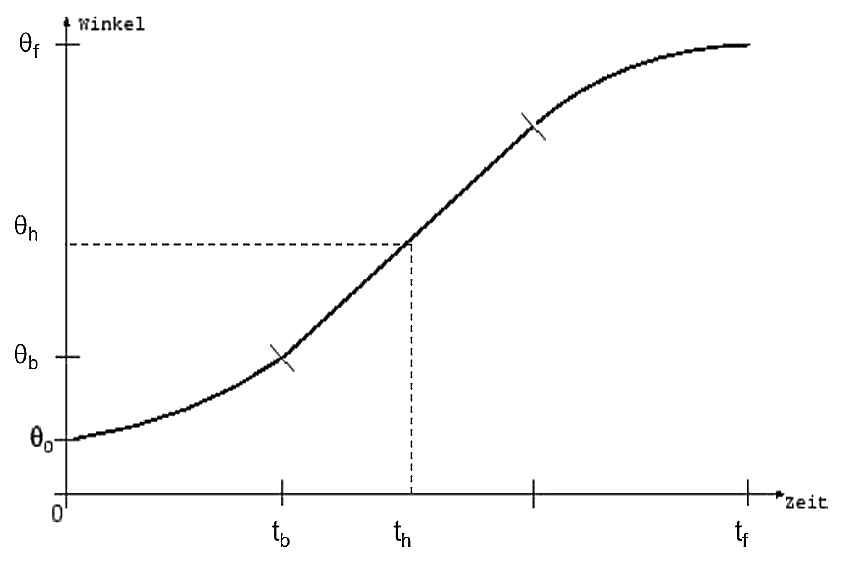
\includegraphics[width=\linewidth]{./bilder/RampenprofilInterpol}
\end{minipage}
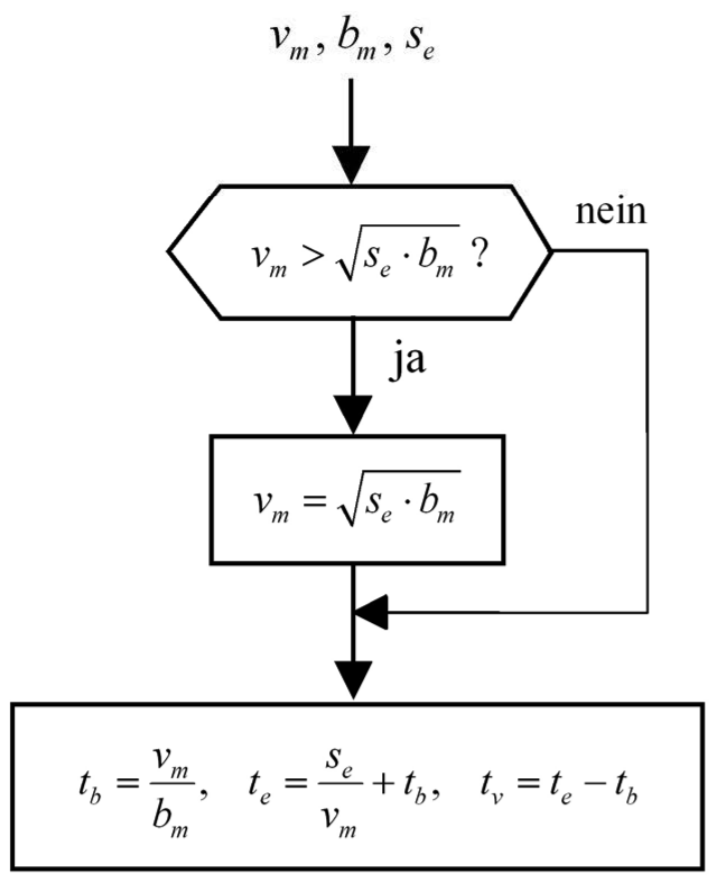
\includegraphics[width=0.25\linewidth]{./bilder/RampenVorgehn}

\subsection{Bahnerzeugungn in karteschien Koordinaten}
\begin{multicols}{2}
    \begin{itemize}
        \item[+] Bahn genau definiert
    \end{itemize}
    
    \begin{itemize}
        \item[-] Berechnung der inv. Koordtrans für jeden Punkt notwendig.
        \item[-] Geometrische Probleme
        \begin{itemize}
            \item Unerreichbare Zwischenpunkte
            \item Hohe v in der näche von Singularitäten
            \item Start/Ziel gehören zu verschiedenen Zweige der kin. Lösung
        \end{itemize}
        \item[-] Schwierig, die Motorenbegrenzung zu berücksichtigen.
    \end{itemize}
\end{multicols}

\begin{minipage}{0.7\linewidth}
    \subsection{Lineare Interpolation}
    \vspace{-0.8cm}
    \[ X_s(t) = X_0 + s(t) \cdot u \]
    \[ u= \frac{x_f - x_0}{||x_f -x_0||} \]
    \[ s(t)=a_0 + a_1 t + a_2 t^2 +a_3t^3 \]
    \[ a_0=0 \quad a_1=0 \quad a_3=\frac{3||x_f-x_0||}{t_f^2} \quad a_3=-\frac{2}{t_f^3}\cdot ||x_f-x_0||  \]
\end{minipage}
\begin{minipage}{0.3\linewidth}
    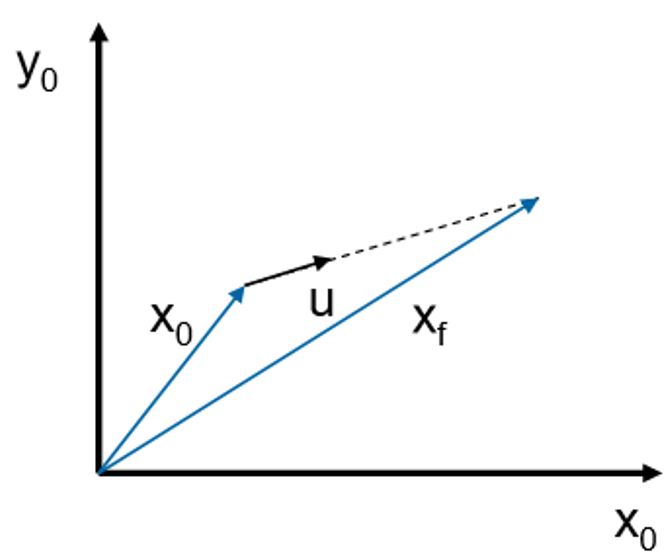
\includegraphics[width=0.9\linewidth]{./bilder/LinInter}
\end{minipage}

\subsection{Vergleich Bahnverläufe}
\begin{multicols}{3}
    \begin{minipage}{\linewidth}
        \subsubsection{Asynchroner PTP}
        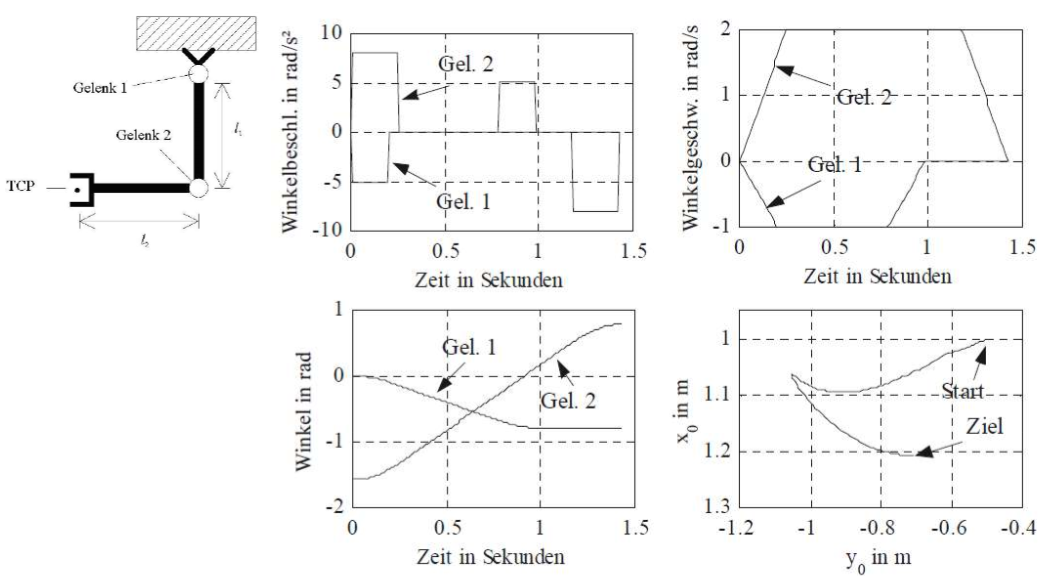
\includegraphics[width=\linewidth]{./bilder/VBAPTP}
    \end{minipage}

    \begin{minipage}{\linewidth}
        \subsubsection{Voll-synchroner PTP}
        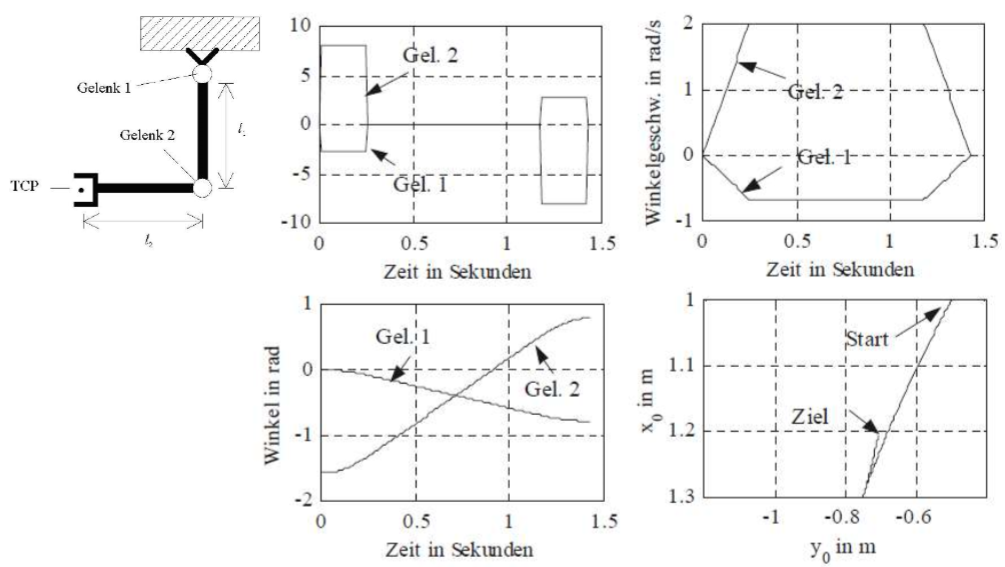
\includegraphics[width=\linewidth]{./bilder/VBVPTP}
    \end{minipage}

    \begin{minipage}{\linewidth}
        \subsubsection{CP-Bahn (linear)}
        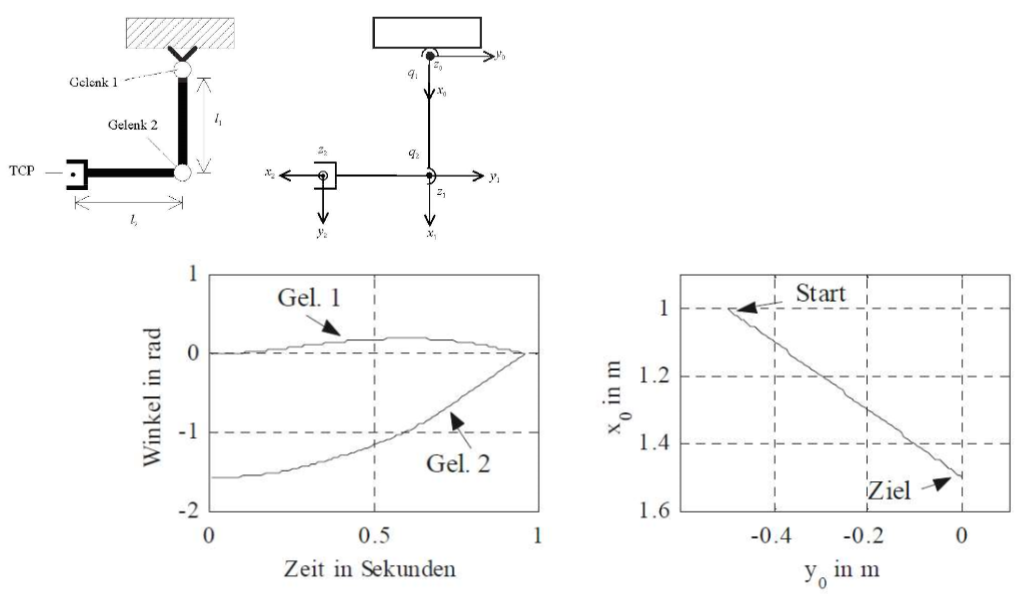
\includegraphics[width=\linewidth]{./bilder/VBCPB}
    \end{minipage}
\end{multicols}

	\subsection{PTP-Synchron}
\begin{minipage}{6cm}
    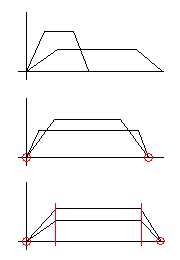
\includegraphics[width=5cm]{./bilder/synchron.png}
\end{minipage}
\begin{minipage}{12.5cm}
    Asynchron PTP\\ \\ \\ \\ \\ \\
    Synchron PTP\\ \\ \\ \\ \\ \\
    Vollsynchron PTP\\
\end{minipage}